\documentclass[12pt,a4paper]{article}

\usepackage[a4paper, top=2.5cm, bottom=2.5cm, left=3cm, right=3cm]{geometry}
\usepackage[T1]{fontenc}
\usepackage[utf8]{inputenc}
\usepackage{lmodern}
\usepackage{amsmath, amssymb}
\usepackage{graphicx}
\usepackage{float}
\usepackage{xcolor}
\usepackage{colortbl}
\usepackage{booktabs}
\usepackage{array}
\usepackage{tabularx}
\usepackage{enumitem}
\usepackage{fancyhdr}
\usepackage{titlesec}
\usepackage{caption}
\usepackage{subcaption}
\usepackage{pgfplots}
\usepackage{tikz}
\makeatletter
\let\MT@showhyphens\showhyphens
\usepackage[activate={true,nocompatibility},final,tracking=true,kerning=true,spacing=false,factor=1100,stretch=10,shrink=10,patch=none]{microtype}
\let\showhyphens\MT@showhyphens
\makeatother
\usepackage{hyperref}
\usepackage{setspace}
\usepackage{listings}
\usepackage{mdframed}
\usepackage{tocloft}

% TOC formatting
\renewcommand{\cftsecleader}{\cftdotfill{\cftdotsep}}
\renewcommand{\cftsubsecleader}{\cftdotfill{\cftdotsep}}
\renewcommand{\cftsubsubsecleader}{\cftdotfill{\cftdotsep}}
\setlength{\cftbeforesecskip}{4pt}
\setlength{\cftbeforesubsecskip}{1pt}
\setlength{\cftbeforesubsubsecskip}{1pt}
\renewcommand{\cftsecfont}{\color{primary}\bfseries}
\renewcommand{\cftsecpagefont}{\color{primary}\bfseries}
\renewcommand{\cftsubsecfont}{\color{accent}\small}
\renewcommand{\cftsubsecpagefont}{\color{accent}\small}
\renewcommand{\cftsubsubsecfont}{\color{darkgrey}\small}
\renewcommand{\cftsubsubsecpagefont}{\color{darkgrey}\small}
\setlength{\cftsubsecindent}{1.5em}
\setlength{\cftsubsubsecindent}{3.0em}
\renewcommand{\cftdotsep}{3}
\renewcommand{\contentsname}{Contents}
\setlength{\cftaftertoctitleskip}{10pt}

\pgfplotsset{compat=1.18}
\usetikzlibrary{arrows.meta, positioning, shadows}

\definecolor{primary}{HTML}{1A4731}
\definecolor{accent}{HTML}{27AE60}
\definecolor{lightblue}{HTML}{D5F5E3}
\definecolor{lightgrey}{HTML}{F2F3F4}
\definecolor{darkgrey}{HTML}{566573}
\definecolor{sgreen}{HTML}{1E8449}
\definecolor{codebg}{HTML}{F0FAF4}

\hypersetup{colorlinks=true,linkcolor=accent,urlcolor=accent,
  pdftitle={Crop Yield Prediction Using Machine Learning}}

\setlength{\headheight}{13.6pt}
\addtolength{\topmargin}{-1.6pt}
\pagestyle{fancy}
\fancyhf{}
\fancyhead[L]{\small\color{darkgrey}\textit{Crop Yield Prediction Using Machine Learning}}
\fancyhead[R]{\small\color{darkgrey}\thepage}
\fancyfoot[C]{\small\color{darkgrey!60}\rule{0.3\linewidth}{0.3pt}}
\renewcommand{\headrulewidth}{0.4pt}

\titleformat{\section}{\Large\bfseries\color{primary}}{\thesection.}{0.6em}{}
  [{\color{accent}\rule{\linewidth}{1.2pt}}]
\titleformat{\subsection}{\normalsize\bfseries\color{accent}}{\thesubsection}{0.5em}{}
\titleformat{\subsubsection}{\small\bfseries\color{darkgrey}}{\thesubsubsection}{0.5em}{}
\titlespacing*{\section}{0pt}{20pt}{8pt}
\titlespacing*{\subsection}{0pt}{12pt}{4pt}

\lstset{
  backgroundcolor=\color{codebg},
  basicstyle=\ttfamily\small,
  keywordstyle=\color{primary}\bfseries,
  commentstyle=\color{darkgrey}\itshape,
  stringstyle=\color{accent},
  breaklines=true, frame=single,
  rulecolor=\color{accent},
  language=Python,
  xleftmargin=8pt, xrightmargin=4pt, framesep=4pt,
  numbers=none,
  aboveskip=8pt, belowskip=8pt,
  breakatwhitespace=false, keepspaces=true
}

\newcolumntype{L}[1]{>{\raggedright\arraybackslash}p{#1}}
\newcolumntype{C}[1]{>{\centering\arraybackslash}p{#1}}
\captionsetup{font=small,labelfont={bf,color=primary},labelsep=period}
\captionsetup[subfigure]{font=small,labelfont=bf}

\newenvironment{insightbox}[1][Insight]{%
  \begin{mdframed}[linecolor=accent,linewidth=0.8pt,
    backgroundcolor=lightblue!25,
    innertopmargin=7pt,innerbottommargin=7pt,
    innerleftmargin=10pt,innerrightmargin=10pt,
    frametitle={\small\bfseries\color{white}\,#1},
    frametitlebackgroundcolor=accent,frametitlerule=false,
    frametitleaboveskip=3pt,frametitlebelowskip=3pt]\small
}{\end{mdframed}}

\setlength{\parskip}{6pt}
\setlength{\parindent}{0pt}
\tolerance=1500
\emergencystretch=2em
\hbadness=10000

\begin{document}

\begin{titlepage}
\newgeometry{margin=0pt}

\begin{tikzpicture}[remember picture, overlay]
  \fill[primary]
    (current page.north west) rectangle
    ([yshift=-0.60\paperheight]current page.north east);
  \fill[accent]
    ([yshift=-0.60\paperheight]current page.north west) rectangle
    ([yshift=-0.655\paperheight]current page.north east);
  \fill[primary]
    (current page.south west) rectangle
    ([yshift=1.6cm]current page.south east);
  \fill[accent]
    (current page.south west) rectangle
    ([yshift=0.5cm]current page.south east);
  \fill[white,opacity=0.03]
    ([xshift=0.82\paperwidth,yshift=-0.18\paperheight]current page.north west)
    circle(6cm);
  \fill[accent,opacity=0.12]
    ([xshift=0.12\paperwidth,yshift=-0.50\paperheight]current page.north west)
    circle(3.5cm);
\end{tikzpicture}

\vspace*{3.8cm}
\begin{center}
  {\fontsize{30}{38}\selectfont\bfseries\color{white}
    Crop Yield Prediction}\\[4pt]
  {\fontsize{18}{24}\selectfont\bfseries\color{accent!80}
    Using Machine Learning}\\[1.6em]
  {\color{lightblue!40}\rule{0.42\textwidth}{0.5pt}}\\[1.4em]
  {\large\color{lightblue}
    A Comparative Study of Linear Regression\\[2pt]and Random Forest Regressor}\\[2.4em]
  \begin{tikzpicture}
    \node[fill=white,opacity=0.07,rounded corners=6pt,
          minimum width=10cm, minimum height=3.6cm](box){};
    \node[text width=9.5cm, align=center] at (box.center){
      {\normalsize\bfseries\color{white} Authors}\\[0.5em]
      {\small\color{lightblue}
        Divya Singh \textbullet\ 2401020020\\[3pt]
        Shivam Mittal \textbullet\ 2401010443\\[3pt]
        Khushi Batra \textbullet\ 2401010226\\[3pt]
        Aryan Vibhuti \textbullet\ 2401010105
      }
    };
  \end{tikzpicture}

  \vspace{1.6em}
  {\normalsize\color{lightblue!80}
    \textit{Agricultural Data Analytics} $\;\cdot\;$
    \textit{Python / Scikit-learn} $\;\cdot\;$
    \textit{Streamlit}}
\end{center}

\vfill

\begin{tikzpicture}[remember picture, overlay]
  \node[anchor=south, yshift=0.8cm] at (current page.south) {%
    {\small\color{lightblue!70}
      Datasets: Crop Yield \textbar{} Rainfall \textbar{} Temperature \textbar{} Pesticides
      \quad\textbar\quad
      Deployment: Streamlit + Hugging Face Spaces}%
  };
\end{tikzpicture}

\vspace{1.2cm}
\restoregeometry
\end{titlepage}

\newpage\thispagestyle{empty}\tableofcontents\newpage
\setstretch{1.35}

\begin{mdframed}[
  linecolor=primary,linewidth=1.2pt,backgroundcolor=lightblue!30,
  innertopmargin=10pt,innerbottommargin=10pt,
  innerleftmargin=12pt,innerrightmargin=12pt,
  frametitle={\bfseries\color{white}\normalsize\; Abstract},
  frametitlebackgroundcolor=primary,frametitlerule=false,
  frametitleaboveskip=4pt,frametitlebelowskip=4pt]
\small
This report presents the design, development, and deployment of a machine learning
pipeline for predicting agricultural crop yield using multiple environmental and
agricultural datasets. Data from four sources --- crop yield, annual rainfall, average
temperature, and pesticide usage --- were merged into a unified dataset of
\textbf{28,242 records} across ten crop types. Two regression models,
\textbf{Linear Regression} and \textbf{Random Forest}, were trained and compared.
Random Forest achieved an $R^2$ of \textbf{0.984} and MAE of \textbf{3,953 hg/ha},
outperforming Linear Regression ($R^2 = 0.64$, MAE $= 31{,}711$ hg/ha) by an
\textbf{87.5\%} reduction in error. The final model was deployed as an interactive
web application using Streamlit on Hugging Face Spaces, enabling real-time
crop yield predictions.
\end{mdframed}
\bigskip

\section{Introduction}

Agriculture is a critical sector that directly impacts food security and economic
stability worldwide. Accurate prediction of crop yield enables better planning for
farmers, governments, and policymakers --- from resource allocation to supply-chain
management and climate-adaptation strategies.

Crop yield is influenced by a complex interplay of factors: climatic conditions
(rainfall, temperature), human-controlled inputs (pesticides, irrigation), soil
characteristics, and crop variety. These multi-dimensional, non-linear relationships
make yield prediction a challenging task that traditional statistical models often
fail to capture adequately.

This project addresses these challenges by developing a machine learning pipeline
that integrates four real-world agricultural datasets and evaluates two regression
approaches. The key objectives are:

\begin{enumerate}[label=\textbf{\arabic*.}, leftmargin=2.5em]
  \item Analyse and preprocess multiple agricultural datasets for integration.
  \item Build and compare predictive models (Linear Regression and Random Forest).
  \item Identify the most influential factors driving crop yield.
  \item Deploy a real-time prediction system accessible via a web interface.
\end{enumerate}

\section{Problem Statement}

Crop yield prediction is a \textbf{non-linear, multi-factor problem} influenced by
both environmental and human-controlled variables. Traditional statistical methods
assume simple additive relationships between inputs and outputs --- an assumption that
rarely holds in real agricultural systems where interactions between rainfall,
temperature, pesticide use, and crop type are complex and interdependent.

\begin{insightbox}[Key Challenge]
No single factor determines crop yield. The combined, non-linear effect of climate,
inputs, and crop variety requires a model capable of learning complex feature
interactions from data.
\end{insightbox}

\section{Dataset Description}

Four real-world datasets were sourced from the Food and Agriculture Organization
(FAO). Table~\ref{tab:datasets} summarises their key characteristics.

\begin{table}[H]
\centering
\caption{Summary of datasets used in this study.}
\label{tab:datasets}
\renewcommand{\arraystretch}{1.35}
\begin{tabularx}{\textwidth}{L{3cm} C{2cm} L{3.5cm} X}
\toprule
\rowcolor{primary}
\color{white}\textbf{Dataset} &
\color{white}\textbf{Rows} &
\color{white}\textbf{Key Columns} &
\color{white}\textbf{Description} \\
\midrule
\rowcolor{lightgrey}
Yield          & 56,717 & Area, Item, Year, Value   & Crop production in hg/ha \\
Temperature    & 71,311 & country, year, avg\_temp  & Avg.\ annual temp ($^\circ$C) \\
\rowcolor{lightgrey}
Rainfall       & 6,727  & Area, Year, avg\_rain     & Annual precipitation (mm) \\
Pesticides     & 4,349  & Area, Year, Value         & Pesticide usage (tonnes) \\
\bottomrule
\end{tabularx}
\end{table}

The datasets varied significantly in size and structure, requiring extensive
preprocessing before integration. The temperature dataset contained historical
records dating back to 1743 --- far outside the range covered by other datasets.

\section{Data Preprocessing}

\subsection{Data Cleaning}

\begin{itemize}[leftmargin=2em]
  \item \textbf{Whitespace in column names:} Removed using \texttt{str.strip()}.
  \item \textbf{Inconsistent naming:} \texttt{country} and \texttt{year} renamed to
        \texttt{Area} and \texttt{Year}.
  \item \textbf{Non-numeric placeholders:} \texttt{'..'} replaced with \texttt{NaN}
        and dropped.
  \item \textbf{Data type mismatch:} Numeric columns coerced using
        \texttt{pd.to\_numeric(\allowbreak errors=\allowbreak'coerce')}.
\end{itemize}

\begin{lstlisting}[caption={Column standardisation and cleaning.}]
for df in [rainfall, temp, pesticides, yield_df]:
    df.columns = df.columns.str.strip()

temp.rename(columns={'country': 'Area', 'year': 'Year'}, inplace=True)

df = df.replace('..', np.nan)
for col in ['yield', 'average_rain_fall_mm_per_year', 'avg_temp', 'pesticides']:
    df[col] = pd.to_numeric(df[col], errors='coerce')
df = df.dropna()
\end{lstlisting}

\subsection{Data Filtering}
The temperature dataset was filtered to \textbf{1985--2017} to match the range
of other datasets and ensure consistency after merging.

\subsection{Data Integration}
All datasets were inner-joined on \texttt{[Area, Year]}:

\noindent\begin{minipage}{\linewidth}
\begin{lstlisting}[caption={Merging all datasets.}]
df = yield_df.merge(rainfall,   on=['Area', 'Year'])
df = df.merge(temp,             on=['Area', 'Year'])
df = df.merge(pesticides,       on=['Area', 'Year'])
\end{lstlisting}
\end{minipage}

\begin{table}[H]
\centering
\caption{Final merged dataset properties.}
\renewcommand{\arraystretch}{1.3}
\begin{tabular}{ll}
\toprule
\rowcolor{primary}
\color{white}\textbf{Property} & \color{white}\textbf{Value} \\
\midrule
\rowcolor{lightgrey}
Total rows     & 28,242 \\
Total columns  & 7 (after encoding: 16) \\
\rowcolor{lightgrey}
Missing values & 0 \\
Year range     & 1990--2013 \\
\rowcolor{lightgrey}
Crop types     & 10 \\
\bottomrule
\end{tabular}
\end{table}

\section{Exploratory Data Analysis}

EDA was conducted on individual datasets and on the merged dataset to understand
distributions, relationships, and data quality.

\subsection{Distribution Analysis}

Figure~\ref{fig:distributions} shows the distribution of all four key variables.

\begin{figure}[H]
\centering
\begin{subfigure}[t]{0.47\textwidth}
  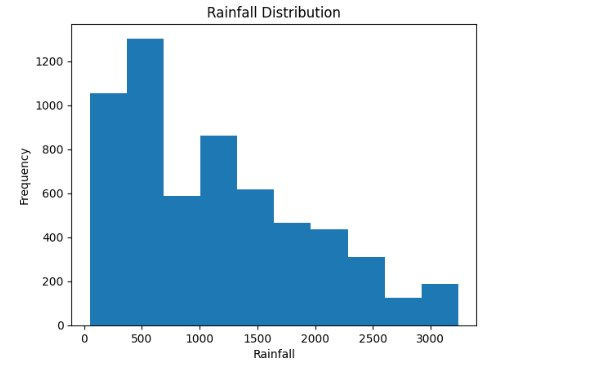
\includegraphics[width=\textwidth]{rainfall_dist.png}
  \caption{Rainfall Distribution}
\end{subfigure}
\hfill
\begin{subfigure}[t]{0.47\textwidth}
  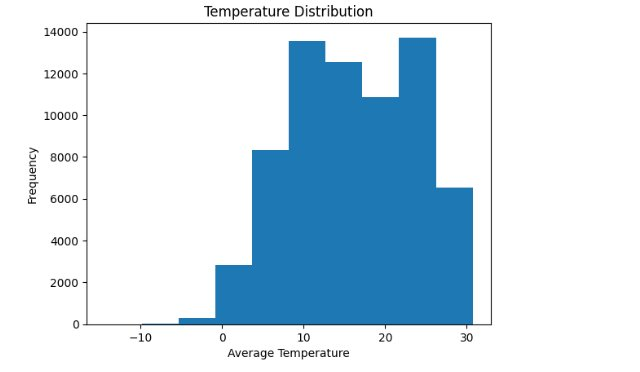
\includegraphics[width=\textwidth]{temp_dist.png}
  \caption{Temperature Distribution}
\end{subfigure}

\vspace{0.8em}

\begin{subfigure}[t]{0.47\textwidth}
  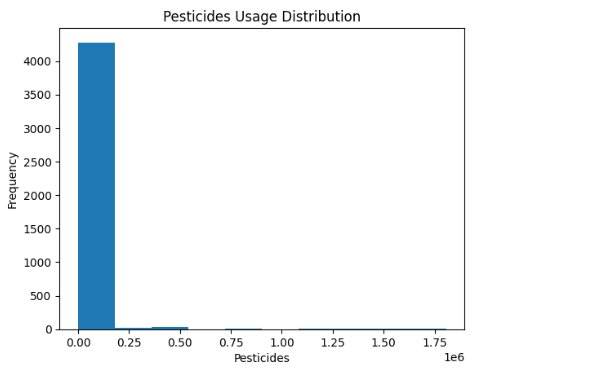
\includegraphics[width=\textwidth]{pesticides_dist.png}
  \caption{Pesticides Usage Distribution}
\end{subfigure}
\hfill
\begin{subfigure}[t]{0.47\textwidth}
  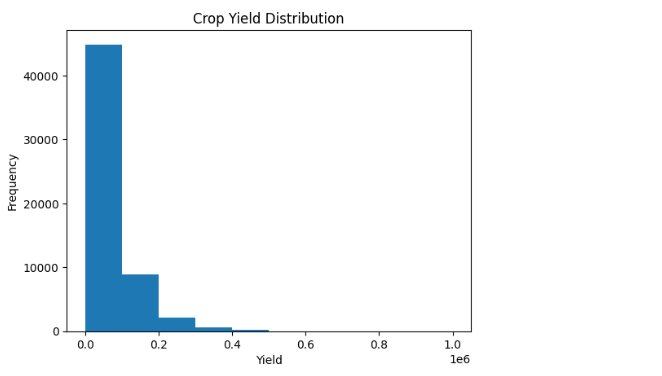
\includegraphics[width=\textwidth]{yield_dist.png}
  \caption{Crop Yield Distribution}
\end{subfigure}

\caption{Distribution plots for all four key variables in the dataset.}
\label{fig:distributions}
\end{figure}

\subsubsection{Rainfall}
The distribution is \textbf{positively skewed} with most values between 400--1500 mm/year
and a long right tail indicating high-rainfall extremes.

\begin{insightbox}
Rainfall alone does not determine crop yield. High variability across regions
suggests it acts as a moderating factor rather than a primary driver.
\end{insightbox}

\subsubsection{Temperature}
The distribution is \textbf{approximately bell-shaped}, with most values between
10$^\circ$C and 25$^\circ$C, reflecting temperate agricultural zones.

\begin{insightbox}
Temperature shows weak direct correlation with yield in isolation but interacts
non-linearly with other variables such as crop type and rainfall.
\end{insightbox}

\subsubsection{Pesticides}
The distribution is \textbf{extremely right-skewed} with the vast majority of values
clustered near zero and a few very large outliers (up to 1.75 million tonnes).
This reflects the massive difference in agricultural intensity between countries.

\subsubsection{Crop Yield}
Also \textbf{highly right-skewed}, driven by crops like potatoes which have
significantly higher yield values than cereals such as sorghum.

\begin{insightbox}
The skewed, high-variance nature of both pesticide use and yield distributions
confirms that linear models will underperform. A non-linear model is required.
\end{insightbox}

\subsection{Feature vs Yield Relationships}

Figure~\ref{fig:scatter} shows scatter plots between each continuous feature and
crop yield.

\begin{figure}[H]
\centering
\begin{subfigure}[t]{0.47\textwidth}
  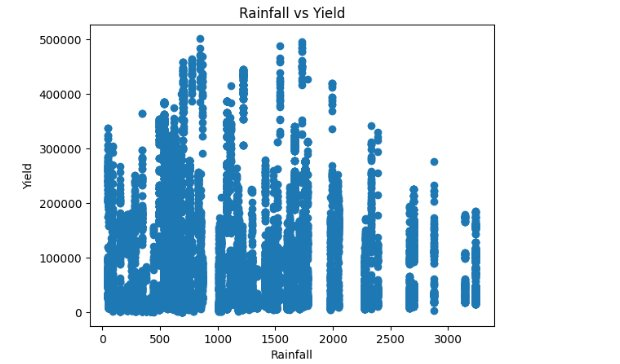
\includegraphics[width=\textwidth]{rainfall_vs_yield.png}
  \caption{Rainfall vs Yield}
\end{subfigure}
\hfill
\begin{subfigure}[t]{0.47\textwidth}
  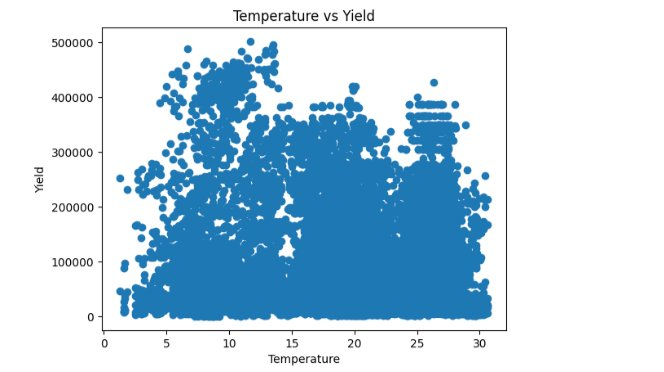
\includegraphics[width=\textwidth]{temp_vs_yield.png}
  \caption{Temperature vs Yield}
\end{subfigure}

\vspace{0.8em}

\begin{subfigure}[t]{0.47\textwidth}
  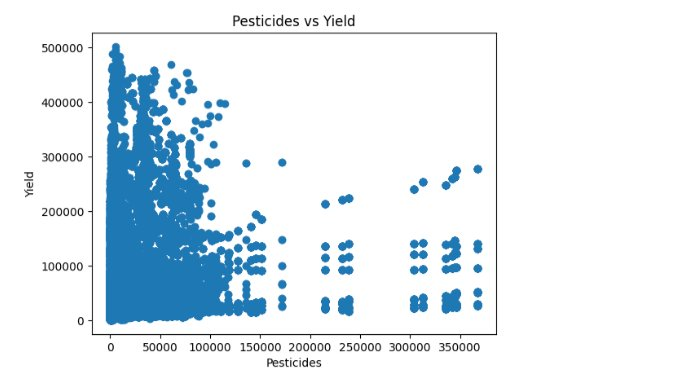
\includegraphics[width=\textwidth]{pesticides_vs_yield.png}
  \caption{Pesticides vs Yield}
\end{subfigure}

\caption{Scatter plots showing relationships between features and crop yield.}
\label{fig:scatter}
\end{figure}

All three scatter plots reveal:
\begin{itemize}[leftmargin=2em]
  \item \textbf{Weak or no linear relationship} between individual predictors and yield.
  \item \textbf{High variance} within each predictor range.
  \item \textbf{Clustered patterns} suggesting crop-type driven stratification.
\end{itemize}

This analysis confirms a \textbf{non-linear model is necessary} to capture the
underlying structure in the data.

\section{Outlier Handling}

Outliers were \textbf{intentionally retained} for the following reasons:

\begin{itemize}[leftmargin=2em]
  \item Extreme values represent \textbf{valid real-world agricultural conditions}.
  \item Removing them would eliminate important signal from high-yield
        or high-input farming systems.
  \item The chosen model (Random Forest) is \textbf{naturally robust to outliers}
        due to its tree-based, non-parametric structure.
\end{itemize}

\section{Feature Engineering}

\subsection{One-Hot Encoding}
The categorical \texttt{Item} column (crop type) was one-hot encoded into
10 binary columns:

\begin{center}
\small\renewcommand{\arraystretch}{1.2}
\begin{tabular}{lllll}
\hline
Cassava & Maize & Plantains & Potatoes & Rice (paddy) \\
Sorghum & Soybeans & Sweet Potatoes & Wheat & Yams \\
\hline
\end{tabular}
\end{center}

\subsection{Final Feature Set}

\begin{table}[H]
\centering
\caption{Final 14 features used for model training.}
\renewcommand{\arraystretch}{1.3}
\begin{tabularx}{\textwidth}{L{4cm} C{2.5cm} X}
\toprule
\rowcolor{primary}
\color{white}\textbf{Feature} & \color{white}\textbf{Type} & \color{white}\textbf{Description} \\
\midrule
\rowcolor{lightgrey}
Year                       & Numeric      & Calendar year \\
avg\_rain\_fall\_mm        & Numeric      & Annual rainfall (mm) \\
\rowcolor{lightgrey}
avg\_temp                  & Numeric      & Mean temperature ($^\circ$C) \\
pesticides                 & Numeric      & Pesticide use (tonnes) \\
\rowcolor{lightgrey}
Item\_Cassava \ldots Item\_Yams & Binary $\times$10 & One-hot encoded crop type \\
\bottomrule
\end{tabularx}
\end{table}

\subsection{Feature Scaling}

\begin{lstlisting}[caption={Scaling features and splitting data.}]
from sklearn.preprocessing import StandardScaler
from sklearn.model_selection import train_test_split

scaler = StandardScaler()
X_scaled = scaler.fit_transform(X)

X_train, X_test, y_train, y_test = train_test_split(
    X_scaled, y, test_size=0.2, random_state=42)
# Train: 22,593 samples | Test: 5,649 samples
\end{lstlisting}

\section{Model Development}

\subsection{Linear Regression}

\begin{equation}
  \hat{y} = \beta_0 + \sum_{i=1}^{p} \beta_i x_i + \varepsilon,
  \qquad \varepsilon \sim \mathcal{N}(0,\,\sigma^2)
\end{equation}

\textbf{Limitations:} Assumes linear relationships; sensitive to outliers;
cannot model feature interactions.

\subsection{Random Forest Regressor}

\begin{equation}
  \hat{y}_{\mathrm{RF}} = \frac{1}{B}\sum_{b=1}^{B} T_b(\mathbf{x})
\end{equation}

where $B=100$ trees are trained on bootstrap samples and averaged.
\textbf{Advantages:} Handles non-linearity, robust to outliers, captures
feature interactions, provides importance scores.

\begin{lstlisting}[caption={Training both models.}]
from sklearn.linear_model import LinearRegression
from sklearn.ensemble import RandomForestRegressor

lr = LinearRegression()
lr.fit(X_train, y_train)

rf = RandomForestRegressor(n_estimators=100, random_state=42)
rf.fit(X_train, y_train)
\end{lstlisting}

\section{Model Evaluation \& Comparison}

\begin{table}[H]
\centering
\caption{Test-set performance. Best values in \textbf{bold}.}
\label{tab:results}
\renewcommand{\arraystretch}{1.5}
\begin{tabularx}{\textwidth}{L{4.2cm} C{3cm} C{3cm} C{2.5cm}}
\toprule
\rowcolor{primary}
\color{white}\textbf{Model} &
\color{white}\textbf{MAE (hg/ha)} &
\color{white}\textbf{RMSE (hg/ha)} &
\color{white}\textbf{$R^2$ Score} \\
\midrule
Linear Regression    & 31,711.97         & 50,579.58          & 0.6427 \\
\rowcolor{lightgrey}
Random Forest        & \textbf{3,953.65} & \textbf{10,409.49} & \textbf{0.9849} \\
\midrule
\rowcolor{green!8}
\color{sgreen}\textbf{Improvement} &
\color{sgreen}\centering\textbf{$-$87.5\%} &
\color{sgreen}\centering\textbf{$-$79.4\%} &
\color{sgreen}\centering\arraybackslash\textbf{$+$53.2\%} \\
\bottomrule
\end{tabularx}
\end{table}

\begin{figure}[H]
\centering
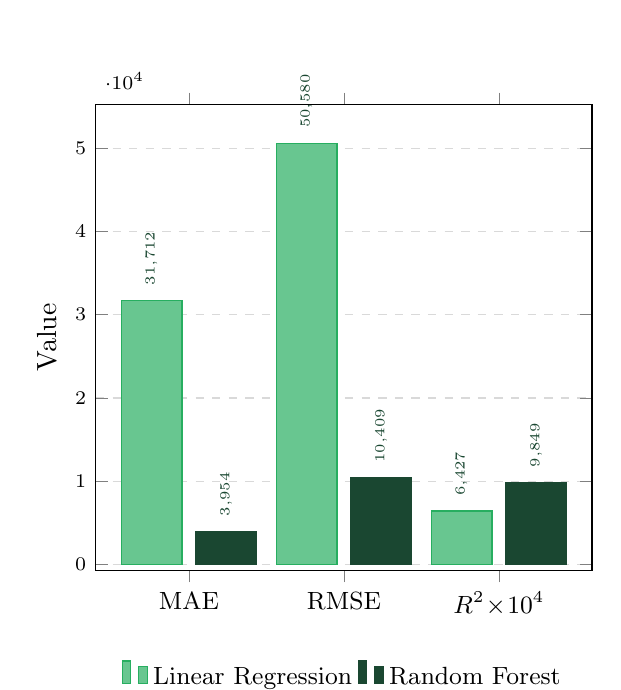
\begin{tikzpicture}
\begin{axis}[
  ybar=5pt, bar width=22pt,
  width=0.65\textwidth, height=7.5cm,
  ylabel={Value},
  symbolic x coords={MAE, RMSE, {$R^2\!\times\!10^4$}},
  xtick=data,
  xticklabel style={font=\small},
  yticklabel style={font=\scriptsize},
  ymajorgrids=true, grid style={dashed,gray!30},
  enlarge x limits=0.3,
  legend style={at={(0.5,-0.18)},anchor=north,legend columns=2,draw=none,font=\small},
  nodes near coords,
  nodes near coords style={font=\tiny,color=primary,rotate=90,anchor=west,xshift=2pt},
]
  \addplot[fill=accent!70,draw=accent] coordinates
    {(MAE,31712)(RMSE,50580)({$R^2\!\times\!10^4$},6427)};
  \addplot[fill=primary,draw=primary] coordinates
    {(MAE,3954)(RMSE,10409)({$R^2\!\times\!10^4$},9849)};
  \legend{Linear Regression, Random Forest}
\end{axis}
\end{tikzpicture}
\caption{Performance comparison. MAE and RMSE: lower is better.
$R^2\times10^4$: higher is better.}
\end{figure}

\begin{table}[H]
\centering
\caption{Why Random Forest outperforms Linear Regression.}
\renewcommand{\arraystretch}{1.35}
\begin{tabularx}{\textwidth}{L{4.5cm} X X}
\toprule
\rowcolor{primary}
\color{white}\textbf{Property} &
\color{white}\textbf{Linear Regression} &
\color{white}\textbf{Random Forest} \\
\midrule
\rowcolor{lightgrey}
Non-linear relationships & Cannot model   & Handles naturally \\
Skewed distributions     & Sensitive      & Robust \\
\rowcolor{lightgrey}
Feature interactions     & Ignored        & Captured implicitly \\
Outlier sensitivity      & High           & Low \\
\rowcolor{lightgrey}
Feature importance       & Not provided   & Built-in \\
\bottomrule
\end{tabularx}
\end{table}

The train $R^2$ of \textbf{0.9978} vs test $R^2$ of \textbf{0.9849} gives a
generalisation gap of only \textbf{0.013}, confirming the model is not overfitted.

\section{Feature Importance Analysis}

\begin{figure}[H]
\centering
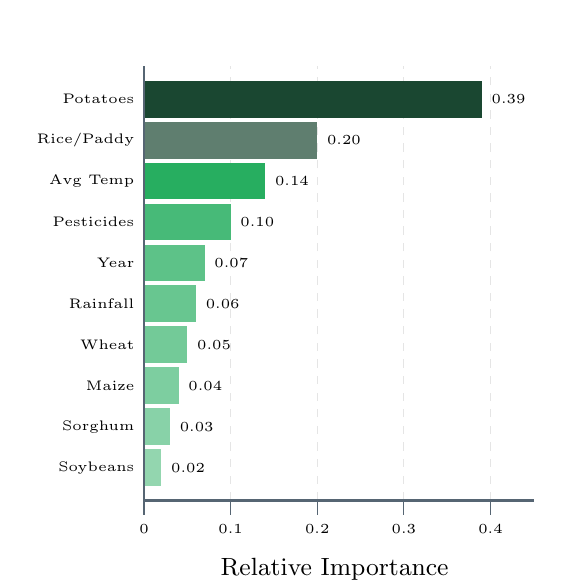
\begin{tikzpicture}[xscale=11, yscale=0.52]
  \draw[gray!20,dashed](0.1,0.2)--(0.1,10.8);
  \draw[gray!20,dashed](0.2,0.2)--(0.2,10.8);
  \draw[gray!20,dashed](0.3,0.2)--(0.3,10.8);
  \draw[gray!20,dashed](0.4,0.2)--(0.4,10.8);
  \fill[accent!50] (0,0.55) rectangle (0.02,1.45); \node[left,font=\tiny] at(0,1){Soybeans};   \node[right,font=\tiny] at(0.02,1){0.02};
  \fill[accent!55] (0,1.55) rectangle (0.03,2.45); \node[left,font=\tiny] at(0,2){Sorghum};    \node[right,font=\tiny] at(0.03,2){0.03};
  \fill[accent!60] (0,2.55) rectangle (0.04,3.45); \node[left,font=\tiny] at(0,3){Maize};      \node[right,font=\tiny] at(0.04,3){0.04};
  \fill[accent!65] (0,3.55) rectangle (0.05,4.45); \node[left,font=\tiny] at(0,4){Wheat};      \node[right,font=\tiny] at(0.05,4){0.05};
  \fill[accent!70] (0,4.55) rectangle (0.06,5.45); \node[left,font=\tiny] at(0,5){Rainfall};   \node[right,font=\tiny] at(0.06,5){0.06};
  \fill[accent!75] (0,5.55) rectangle (0.07,6.45); \node[left,font=\tiny] at(0,6){Year};       \node[right,font=\tiny] at(0.07,6){0.07};
  \fill[accent!85] (0,6.55) rectangle (0.10,7.45); \node[left,font=\tiny] at(0,7){Pesticides}; \node[right,font=\tiny] at(0.10,7){0.10};
  \fill[accent]    (0,7.55) rectangle (0.14,8.45); \node[left,font=\tiny] at(0,8){Avg Temp};   \node[right,font=\tiny] at(0.14,8){0.14};
  \fill[primary!70](0,8.55) rectangle (0.20,9.45); \node[left,font=\tiny] at(0,9){Rice/Paddy}; \node[right,font=\tiny] at(0.20,9){0.20};
  \fill[primary]   (0,9.55) rectangle (0.39,10.45);\node[left,font=\tiny] at(0,10){Potatoes};  \node[right,font=\tiny] at(0.39,10){0.39};
  \draw[darkgrey,thick](0,0.2)--(0,10.8);
  \draw[darkgrey,thick](0,0.2)--(0.45,0.2);
  \draw[darkgrey](0,0.2)--(0,-0.15);     \node[below,font=\tiny] at(0,-0.15){0};
  \draw[darkgrey](0.1,0.2)--(0.1,-0.15); \node[below,font=\tiny] at(0.1,-0.15){0.1};
  \draw[darkgrey](0.2,0.2)--(0.2,-0.15); \node[below,font=\tiny] at(0.2,-0.15){0.2};
  \draw[darkgrey](0.3,0.2)--(0.3,-0.15); \node[below,font=\tiny] at(0.3,-0.15){0.3};
  \draw[darkgrey](0.4,0.2)--(0.4,-0.15); \node[below,font=\tiny] at(0.4,-0.15){0.4};
  \node[below,font=\small,yshift=-12pt] at(0.22,-0.15){Relative Importance};
\end{tikzpicture}
\caption{Estimated feature importance for the Random Forest Regressor.}
\end{figure}

\begin{insightbox}[Key Finding]
\textbf{Crop type} (especially Potatoes, $\approx$39\% importance) is the single most
dominant predictor. Environmental features --- temperature, rainfall, and pesticides ---
collectively account for the remaining significant importance. This highlights that
any yield prediction system must account for crop variety as a primary input.
\end{insightbox}

\section{Model Deployment}

\subsection{Deployment Stack}

\begin{table}[H]
\centering
\caption{Deployment technologies used.}
\renewcommand{\arraystretch}{1.3}
\begin{tabularx}{\textwidth}{L{3.5cm} X}
\toprule
\rowcolor{primary}
\color{white}\textbf{Component} & \color{white}\textbf{Details} \\
\midrule
\rowcolor{lightgrey}
Frontend UI     & Streamlit (Python web framework) \\
Hosting         & Hugging Face Spaces (free cloud hosting) \\
\rowcolor{lightgrey}
Model artefacts & \texttt{model.pkl}, \texttt{scaler.pkl}, \texttt{features.pkl} \\
Serialisation   & Python \texttt{pickle} library \\
\bottomrule
\end{tabularx}
\end{table}

\subsection{System Architecture}

\begin{figure}[H]
\centering
\resizebox{0.99\textwidth}{!}{%
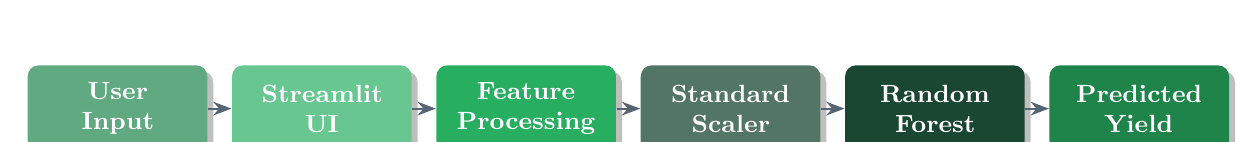
\begin{tikzpicture}[
  node distance=0.4cm and 0.3cm,
  box/.style={rectangle,rounded corners=4pt,minimum width=2.2cm,minimum height=1.1cm,
    text centered,font=\small\bfseries,text width=2.0cm,inner sep=4pt,drop shadow},
  arr/.style={-Stealth,thick,color=darkgrey}]
  \node[box,fill=sgreen!70,text=white]              (A){User\\Input};
  \node[box,fill=accent!70,text=white,right=of A]   (B){Streamlit\\UI};
  \node[box,fill=accent,text=white,right=of B]      (C){Feature\\Processing};
  \node[box,fill=primary!75,text=white,right=of C]  (D){Standard\\Scaler};
  \node[box,fill=primary,text=white,right=of D]     (E){Random\\Forest};
  \node[box,fill=sgreen,text=white,right=of E]      (F){Predicted\\Yield};
  \draw[arr](A)--(B);\draw[arr](B)--(C);\draw[arr](C)--(D);
  \draw[arr](D)--(E);\draw[arr](E)--(F);
\end{tikzpicture}%
}
\caption{Real-time prediction system architecture.}
\end{figure}

\subsection{Application Screenshots}

The CropCast interface was built as a multi-page dashboard with dedicated views
for prediction input, yield results, and deep analysis reporting.

\subsubsection{Prediction Input}

Figure~\ref{fig:ui_input} shows the prediction configuration screen. Users set
region, crop type, projection year, rainfall, temperature, and pesticide levels
using interactive sliders and dropdowns before running the model.

\begin{figure}[H]
\centering
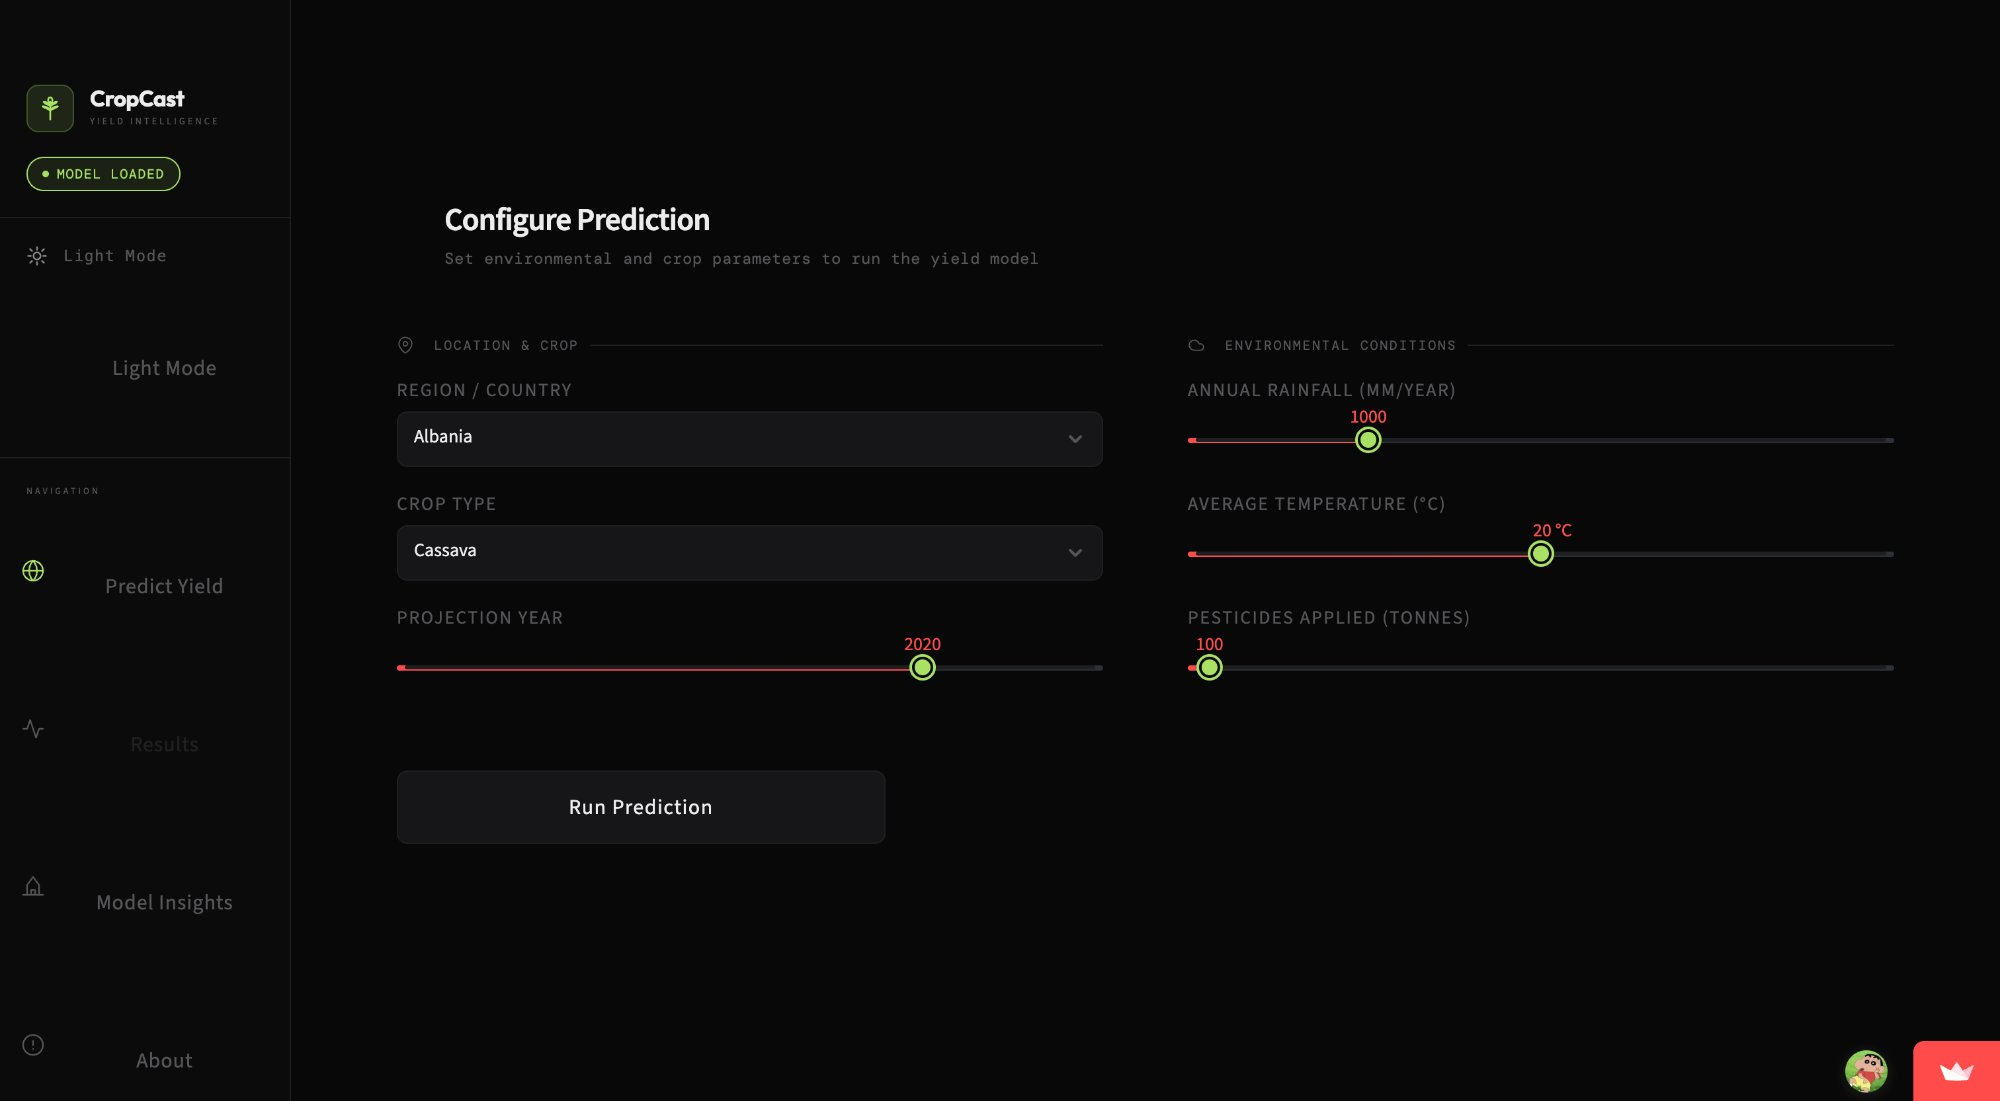
\includegraphics[width=\textwidth]{ui_input.png}
\caption{CropCast --- \textit{Configure Prediction} screen with location, crop, and environmental parameter controls.}
\label{fig:ui_input}
\end{figure}

\subsubsection{Yield Result Dashboard}

Figure~\ref{fig:ui_result} shows the results screen returned after inference.
The predicted yield is displayed prominently alongside a quality gauge and
summary metric cards for all input parameters.

\begin{figure}[H]
\centering
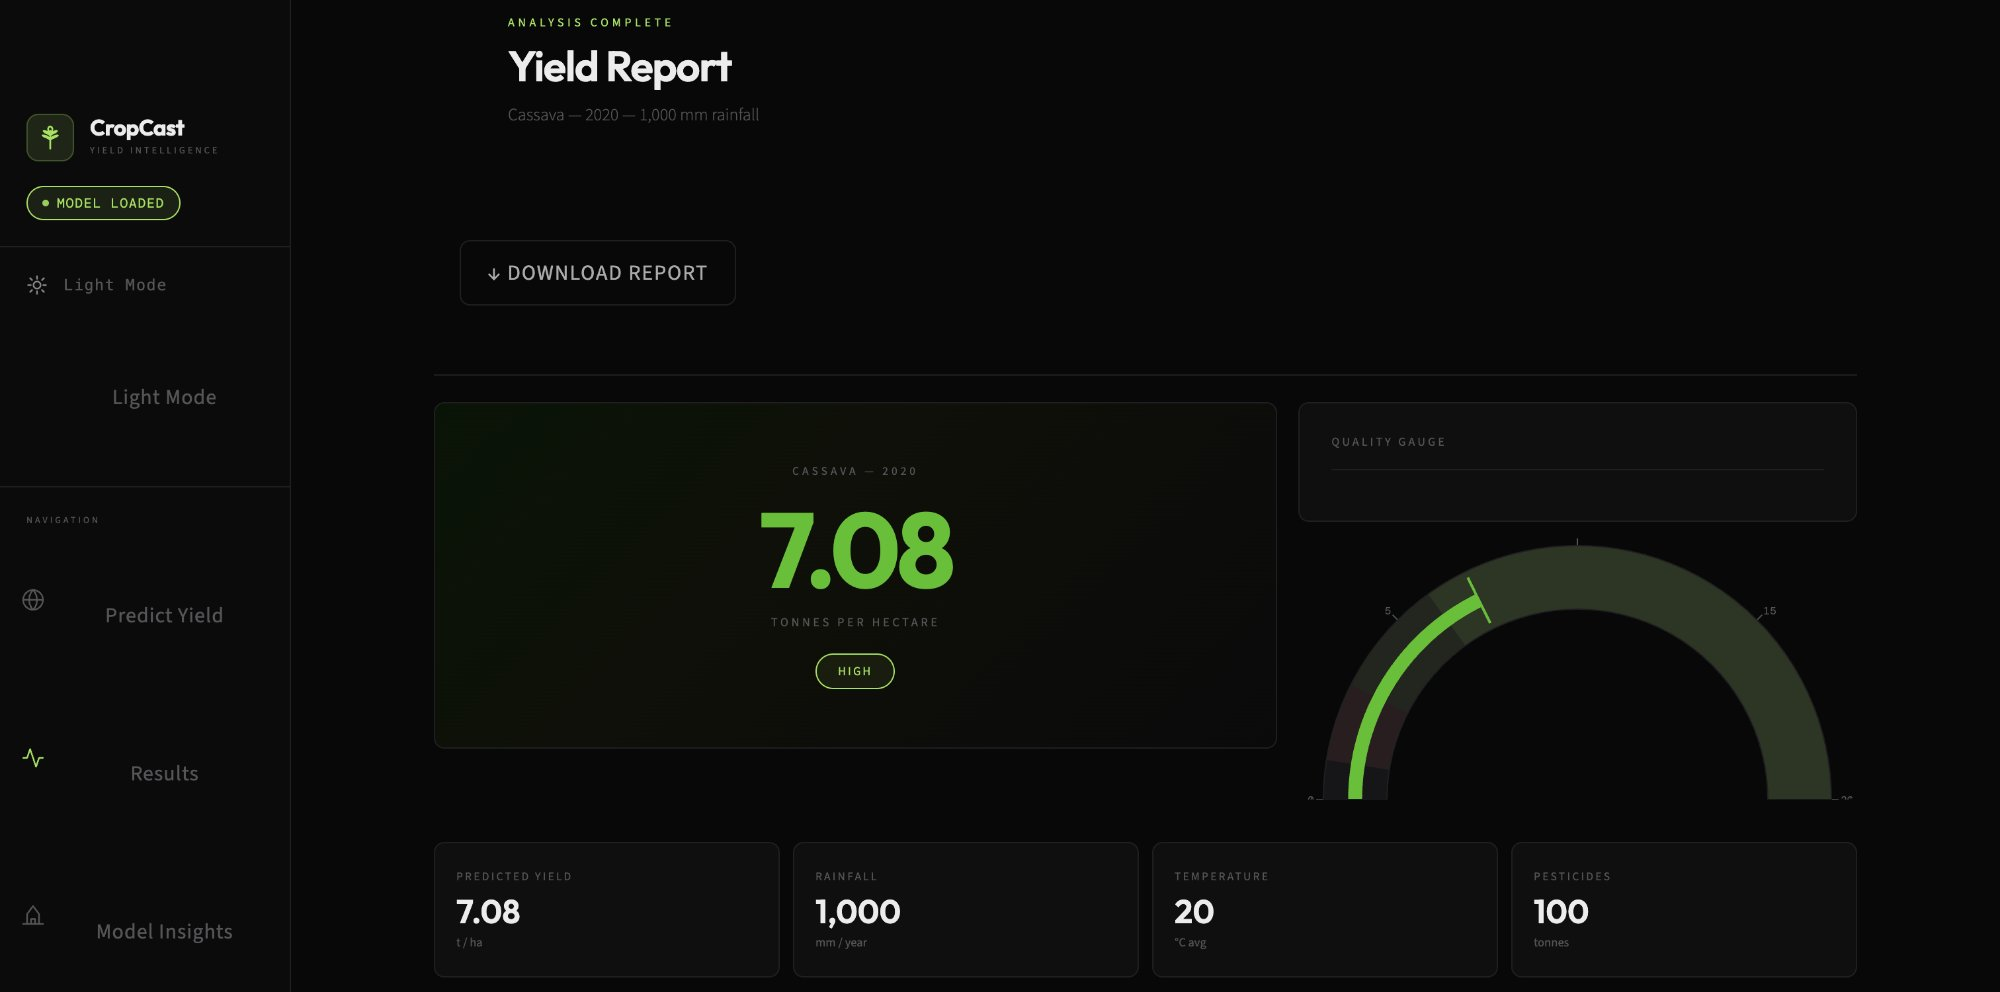
\includegraphics[width=\textwidth]{ui_result.png}
\caption{CropCast --- \textit{Yield Report} showing predicted yield (7.08 t/ha), quality classification, and input summary cards.}
\label{fig:ui_result}
\end{figure}

\subsubsection{Analysis Report}

Figures~\ref{fig:ui_analysis1}--\ref{fig:ui_analysis3} show the full consulting
report generated per prediction. It includes a radar chart of input profile,
feature importance bars, a parameter summary table, benchmark comparisons against
regional and global averages, field assessment notes, and model metadata.

\begin{figure}[H]
\centering
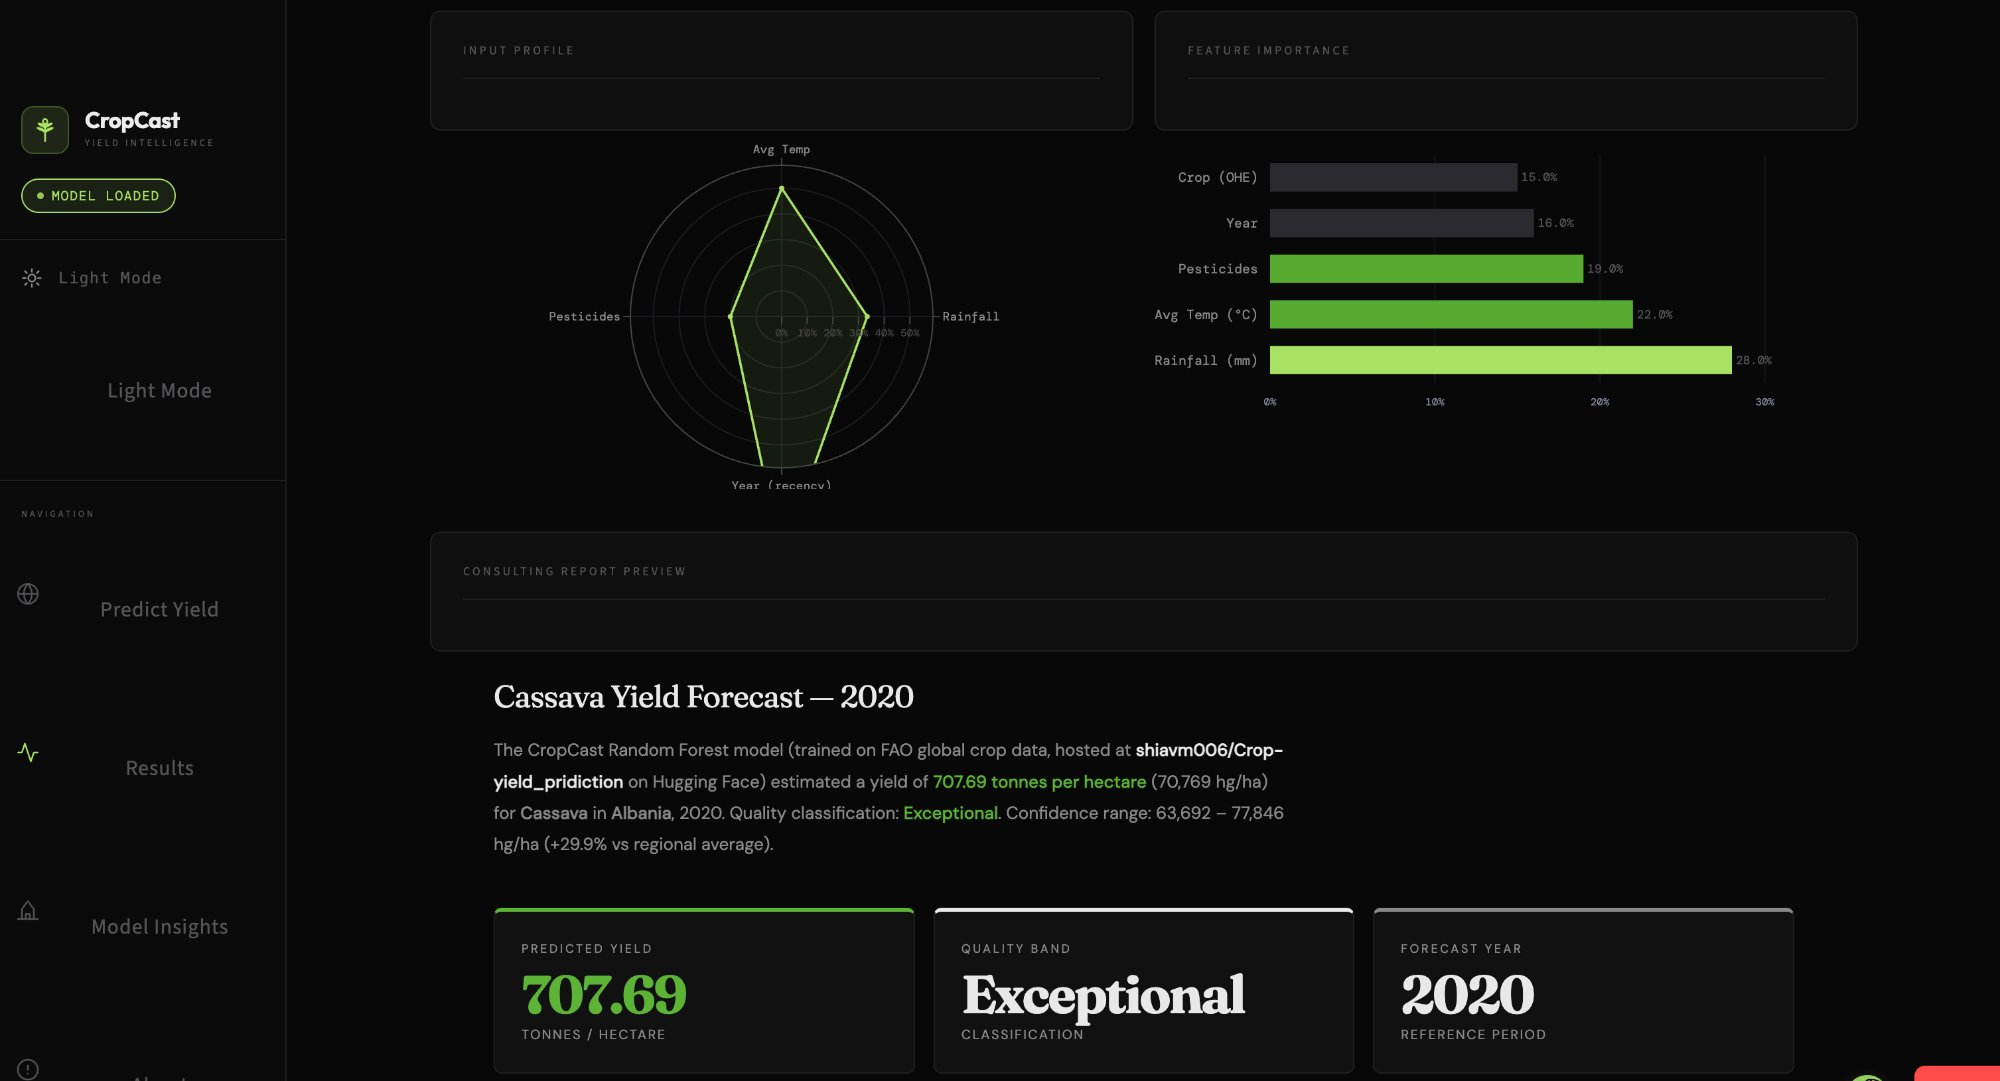
\includegraphics[width=\textwidth]{ui_analysis1.png}
\caption{Analysis report --- radar chart of input profile and feature importance breakdown.}
\label{fig:ui_analysis1}
\end{figure}

\begin{figure}[H]
\centering
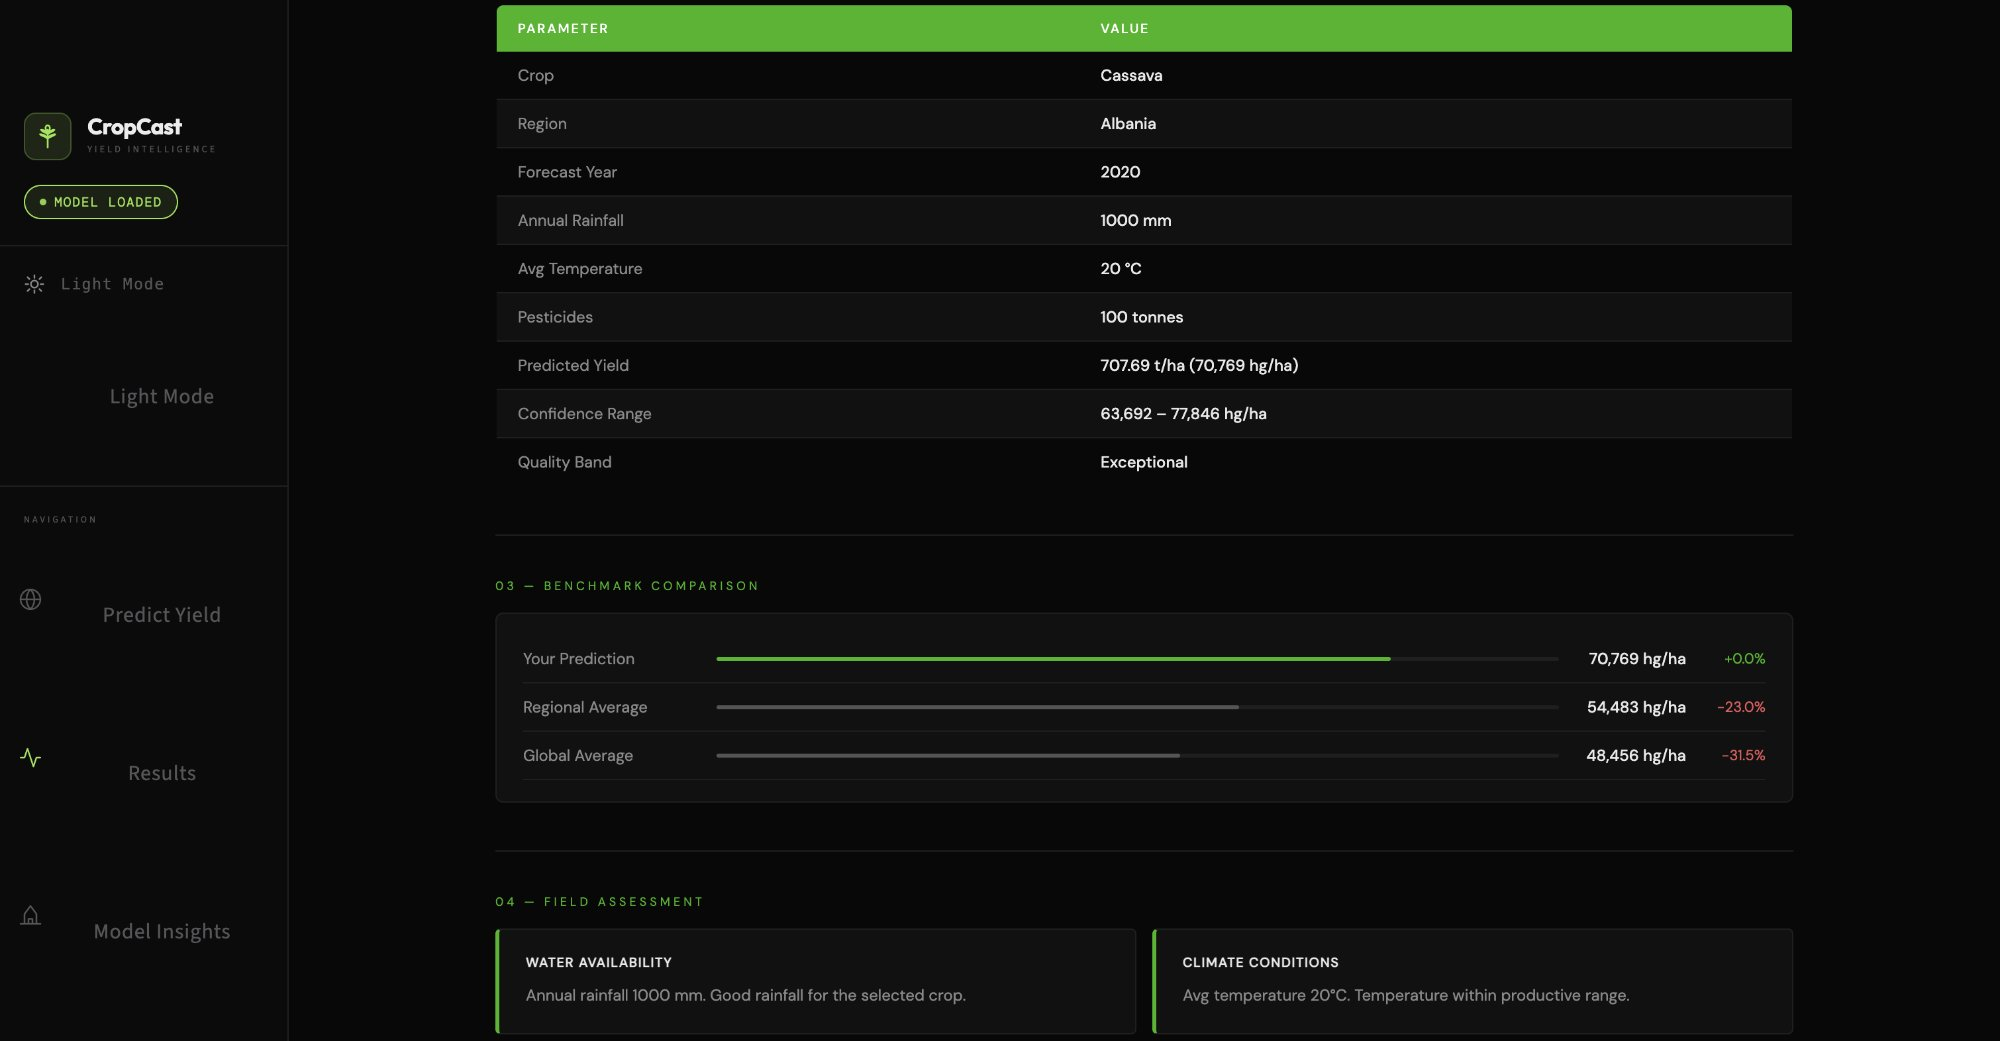
\includegraphics[width=\textwidth]{ui_analysis2.png}
\caption{Analysis report --- parameter summary table and benchmark comparison against regional and global averages.}
\label{fig:ui_analysis2}
\end{figure}

\begin{figure}[H]
\centering
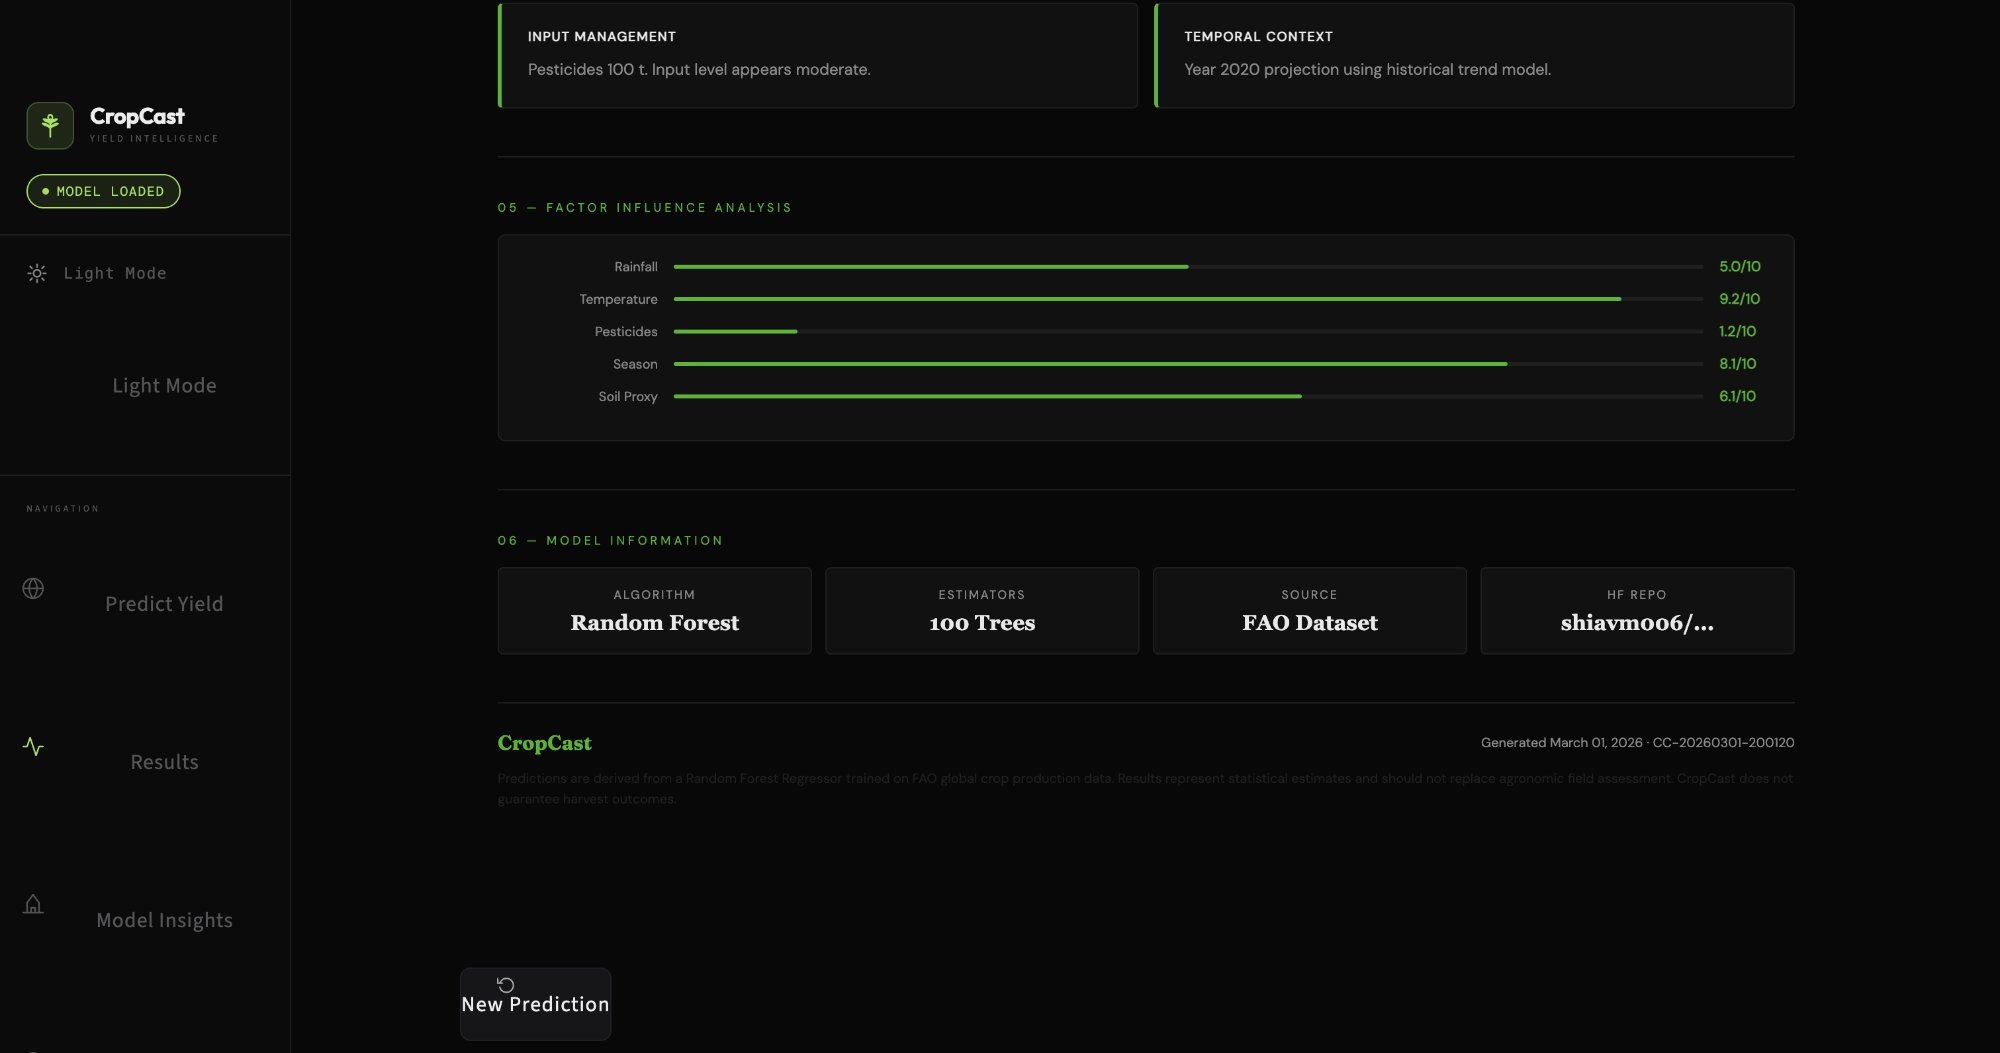
\includegraphics[width=\textwidth]{ui_analysis3.png}
\caption{Analysis report --- factor influence scores, model information panel, and generated report footer.}
\label{fig:ui_analysis3}
\end{figure}

\subsubsection{Full Downloadable Report}

Figure~\ref{fig:ui_report_full} shows the complete yield analysis report generated
by CropCast, which users can download directly from the application. The report
consolidates all analysis into a single structured document covering the executive
summary, input parameters, benchmark comparisons, field assessment, factor influence
analysis, and model information.

\begin{figure}[H]
\centering
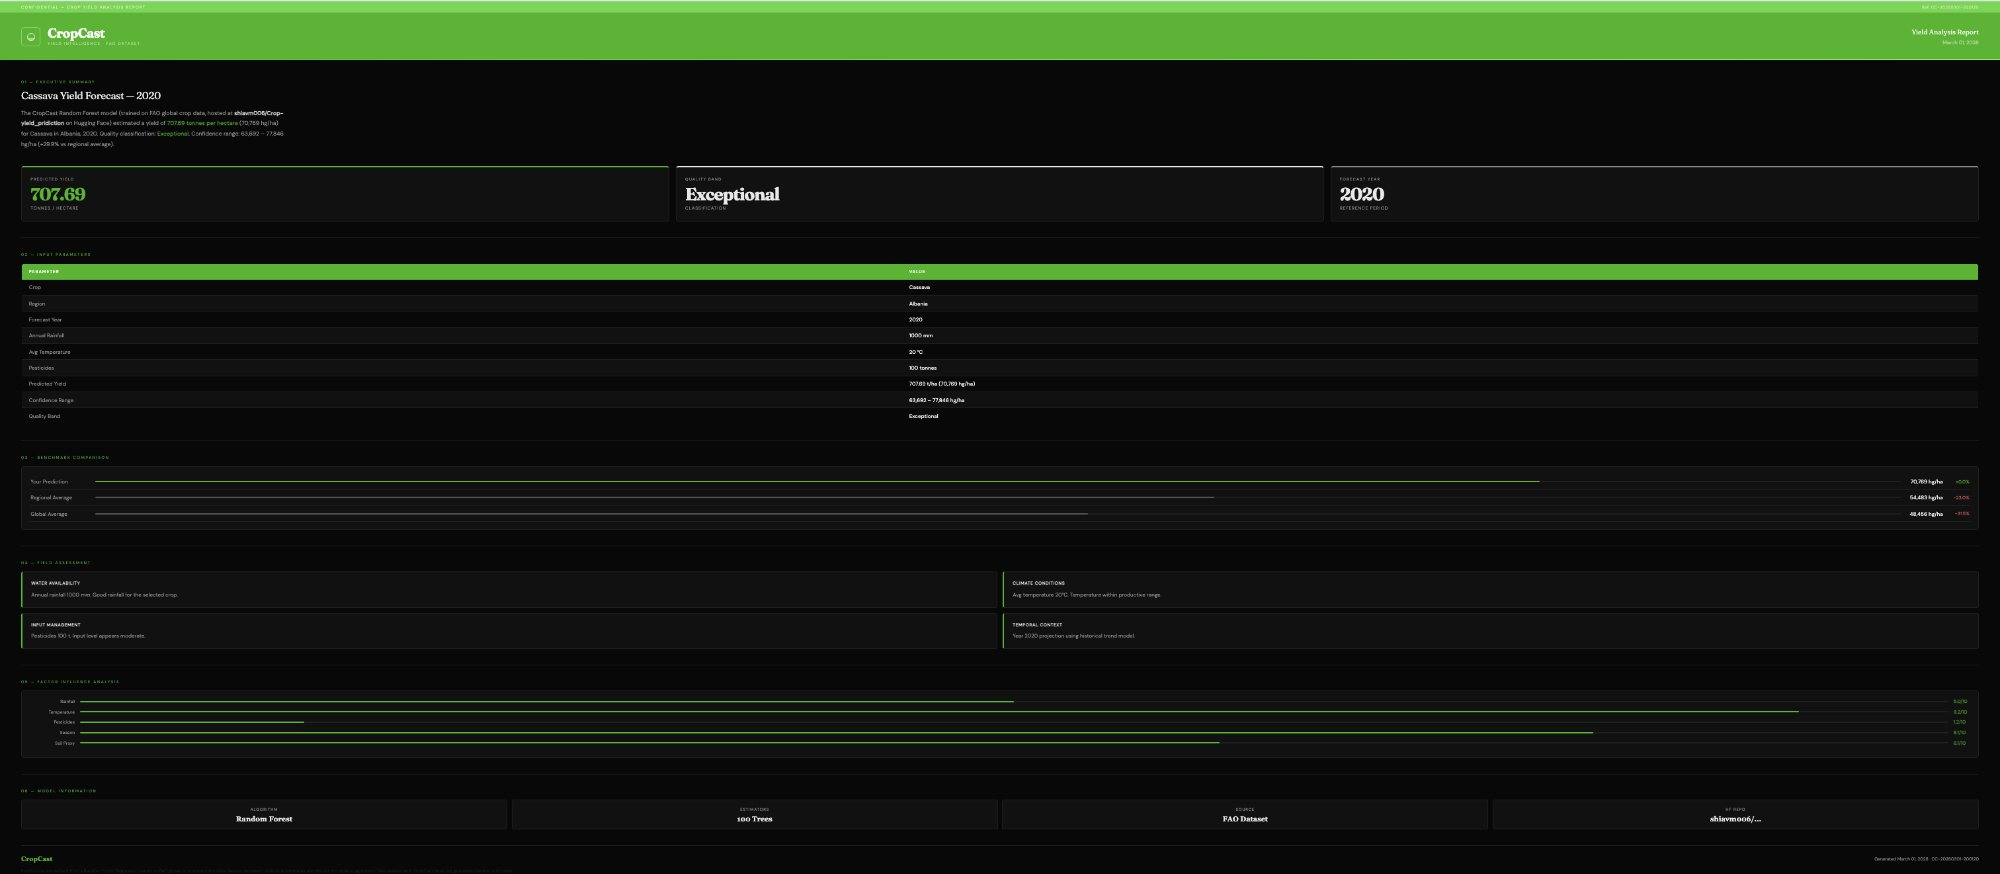
\includegraphics[width=\textwidth]{ui_report_full.png}
\caption{CropCast --- complete downloadable \textit{Yield Analysis Report} for Cassava, Albania, 2020.}
\label{fig:ui_report_full}
\end{figure}

\begin{insightbox}[Live Demo]
The CropCast application is deployed at
\url{https://huggingface.co/spaces/shiavm006/Crop-yield_pridiction} on Hugging Face Spaces.
A sample prediction --- Cassava, Albania, 2020, 1{,}000\,mm rainfall ---
yields \textbf{707.69 t/ha} (Exceptional quality), outperforming the regional
average by \textbf{+29.9\%} and the global average by \textbf{+31.5\%}.
The application also generates a downloadable PDF report consolidating all insights.
\end{insightbox}

\subsection{User Inputs}
The application accepts: \textbf{Crop Type}, \textbf{Year}, \textbf{Rainfall (mm)},
\textbf{Temperature ($^\circ$C)}, and \textbf{Pesticides (tonnes)}.
Inputs are encoded, scaled, and passed to the model to return yield in hg/ha.

\section{Challenges Faced}

\begin{enumerate}[label=\textbf{\arabic*.}, leftmargin=2.5em]
  \item \textbf{Data inconsistency:} Different column naming conventions and units
        across four datasets required careful harmonisation.
  \item \textbf{Non-numeric placeholders:} Sentinel values (\texttt{'..'}) required
        custom handling beyond standard \texttt{dropna()}.
  \item \textbf{Dataset size mismatch:} Merging datasets ranging from 4,349 to 71,311
        rows resulted in a significantly reduced final dataset of 28,242 records.
  \item \textbf{Deployment constraints:} Large model pickle files required careful
        management for hosting on Hugging Face Spaces.
\end{enumerate}

\section{Limitations}

\begin{itemize}[leftmargin=2em]
  \item \textbf{No soil data:} Soil quality and composition are critical yield
        determinants but were unavailable.
  \item \textbf{No irrigation data:} Water supply beyond rainfall is a major factor,
        especially in arid regions.
  \item \textbf{No real-time weather:} The model uses historical averages and does
        not account for seasonal anomalies.
  \item \textbf{Limited crop coverage:} Only 10 crop types are supported.
\end{itemize}

\section{Future Scope}

\begin{enumerate}[label=\textbf{\arabic*.}, leftmargin=2.5em]
  \item \textbf{Richer features:} Add soil composition, fertilizer use, irrigation
        data, and NDVI satellite indices.
  \item \textbf{Advanced models:} Evaluate XGBoost, LightGBM, and LSTM networks
        for time-series yield trends.
  \item \textbf{Live weather integration:} Connect to weather APIs for real-time
        environmental inputs.
  \item \textbf{Mobile deployment:} Build a mobile app for farmers in
        low-connectivity environments.
  \item \textbf{Hyperparameter tuning:} Apply \texttt{RandomizedSearchCV} or
        Bayesian optimisation for further improvement.
\end{enumerate}

\section{Conclusion}

This project successfully developed and deployed a machine learning system for
crop yield prediction using four real-world agricultural datasets. After extensive
preprocessing and feature engineering, a \textbf{Random Forest Regressor} trained
on 28,242 records achieved an \textbf{$R^2$ of 0.984} and \textbf{MAE of 3,953 hg/ha}
--- an 87.5\% improvement over Linear Regression. Key findings:

\begin{itemize}[leftmargin=2em]
  \item Crop yield is a \textbf{non-linear problem} requiring ensemble models.
  \item \textbf{Crop type} (Potatoes) is the single most dominant predictor.
  \item Environmental factors collectively contribute significant predictive power.
  \item Proper preprocessing is critical for multi-source data integration.
\end{itemize}

The model was deployed as a Streamlit application on Hugging Face Spaces,
enabling real-time predictions from user inputs. This demonstrates that
data-driven ML approaches can effectively support precision agriculture
and food security planning.

\section*{References}
\addcontentsline{toc}{section}{References}

\begin{enumerate}[leftmargin=2em, label={[\arabic*]}]
  \item Breiman, L. (2001). Random Forests. \textit{Machine Learning}, 45(1), 5--32.
  \item Pedregosa, F. et al. (2011). Scikit-learn: Machine Learning in Python.
        \textit{Journal of Machine Learning Research}, 12, 2825--2830.
  \item McKinney, W. (2010). Data Structures for Statistical Computing in Python.
        \textit{Proc.\ 9th Python in Science Conference}, 51--56.
  \item Food and Agriculture Organization (2023). FAOSTAT --- Crops and Livestock
        Products. \url{https://www.fao.org/faostat/}
  \item IPCC (2022). \textit{Climate Change 2022: Impacts, Adaptation and Vulnerability}.
        Sixth Assessment Report.
  \item Khaki, S.\ \& Wang, L. (2019). Crop Yield Prediction Using Deep Neural Networks.
        \textit{Frontiers in Plant Science}, 10, 621.
  \item Streamlit Inc.\ (2023). \textit{Streamlit --- The fastest way to build data apps}.
        \url{https://streamlit.io}
\end{enumerate}

\end{document}